\documentclass[12pt]{article}

\usepackage{graphicx}
\usepackage[french]{babel}
\usepackage[utf8]{inputenc}

%%%%%%%%%%%%%%%% Lengths %%%%%%%%%%%%%%%%
\setlength{\textwidth}{15.5cm}
\setlength{\evensidemargin}{0.5cm}
\setlength{\oddsidemargin}{0.5cm}

%%%%%%%%%%%%%%%% Variables %%%%%%%%%%%%%%%%

\def\titre{Ordonnanceur de threads}
\def\equipe{Romain BESNARD\\ Amandine GEORGES\\ Lun JIANG\\ Quentin LAMBERT}


\begin{document}

%%%%%%%%%%%%%%%% Header %%%%%%%%%%%%%%%%
\fbox{
  \noindent\begin{minipage}{0.98\textwidth}
  \vskip 0mm
  \noindent
      { \begin{tabular}{p{7.5cm}}
          {\bfseries \sffamily
            Projet de système d'exploitation} \\
          {\itshape \titre}
      \end{tabular}}
      \hfill
      \fbox{\begin{tabular}{l}
          {~\hfill \bfseries \sffamily Equipe :
            \hfill~} \\[2mm]
          \equipe \\

      \end{tabular}}
      \vskip 4mm ~

      ~~~\parbox{0.95\textwidth}{\small \textit{Résumé~:} \sffamily Le
        projet qui nous a été proposé consiste en l'implémentation
        d'un ordonnanceur de threads. Nous étions tenus dans un
        premier temps d'implémenter des fonctions de base assurant 
        le bon fonctionnement d'un code exemple qui nous était fourni.
		
		Nous avons par la suite ajouté des fonctionnalités
		supplémentaires telles qu'une gestion de priorité, de signaux 
		ou bien une préemption forçant un thread de laisser la main
		si il l'a depuis trop longtemps.         
        }

      \vskip 1mm ~

  \end{minipage}
}

~~\\
~~\\

\input{intro.tex}
\section {La structure thread}

Un type \verb'thread_t' devait être implémenté pour correspondre à
l'exemple, nous avons décidé qu'il représenterait un pointeur vers une
structure thread que nous allons maintenant détailler.\\

\begin{verbatim}
struct thread {
    ucontext_t uc;
    void *retval;
    struct GList * sleeping_list;

    treat_func treat_tab[NB_SIG];
    GList* sig_list;

    /*valgrind stackid*/
    int stackid;
}
\end{verbatim}
% à mettre à jour
Le champ \verb'uc' sert à conserver le contexte d'exécution du thread,
\verb'retval' quant à lui permet de stocker la valeur de retour d'un
thread quand celui-ci est dans la liste "zombie". Mais quand il
est dans la liste "ready", \verb'retval' peut contenir la valeur de retour du
thread qu'il attendait. Le dernier champ est la liste des
threads dormants dans l'attente de la fin de l'exécution de ce thread.

\section {Les threads dans l'état "ready" et "zombie"}

Nous avons choisi de stocker ces threads dans deux listes distinctes
pour chacun des états. Les threads "ready" sont ceux prêts à
s'exécuter, et les threads "zombie" ont terminé leur exécution et
attendent que leur valeur de retour soit récupérée.\\ Nous avons pris
comme convention que la tête de la liste "ready" soit le thread en
cours d'exécution.

\section {Utilisation de la GLib}

Pour nous abstraire de l'implémentation du TAD list nous avons utilisé
la GLib, nous fournissant les fonctions nécessaires à la manipulation
des listes de threads tout en nous assurant qu'il n'y aura aucune
fuite mémoire.

\section {L'implémentation des fonctions}

\begin{verbatim}
thread_t thread_self(void);
\end{verbatim}
Avec notre choix de mettre le thread courant en tête de la liste "ready",
cette fonction renvoie simplement la tête de la liste "ready".
~~\\
\begin{verbatim}
int thread_create(thread_t *newthread, void *(*func)(void *), void *funcarg);
\end{verbatim}


Cette fonction a la responsablité d'ajouter le thread main dans la
liste "ready", si c'est la première fois qu'on crée un thread.  Comme
la liste "ready" est initialement vide, la fonction vérifie si cette
liste est vide, et si c'est le cas, elle alloue une instance de la
structure thread, sauvegarde le contexte du main dans cette instance
et la place à la tête de la liste.  Puis elle crée une instance de la
structure thread avec la fonction passée en paramètre et retourne un
thread\_t pointant sur cette structure.  ~~\\
\begin{verbatim}
int thread_yield(void);
\end{verbatim}
Cette fonction fait un $swapcontext$ sur le contexte de la tête de la
liste "ready" (qui est le thread courant) et celui de l'élément
suivant.  ~~\\
\begin{verbatim}
int thread_join(thread_t thread, void **retval);
\end{verbatim}
Cette fonction vérifie tout d'abord si le thread qu'on veut attendre
est dans la liste "ready". Si c'est le cas alors elle se met dans la
liste des dormants de ce thread et passe la main au suivant.  Sinon
elle vérifie si ce thread est dans la liste "zombie", auquel cas
elle prend la valeur de retour de ce thread et continue son exécution.
Enfin si ce thread n'est pas dans la liste "zombie" alors elle
retourne -1 pour dire que l'appel a échoué et que ce thread n'existe
pas.  ~~\\
\begin{verbatim}
void thread_exit(void *retval);
\end{verbatim}
Cette fonction réveille tous les threads de sa liste des dormants et
met à jour son champ retval avec la valeur en paramètre. Puis elle se
met dans la liste "zombie" et passe la main au suivant.

\section{Ordonnancement des threads}
Deux politiques d'ordonnancement a été implémentées.  La première est
du type FIFO et la deuxième utilise la priorité des threads.

L'ordonnancement du type FIFO ajoute simplement les nouveaux threads
ou ceux qui ont laissé la main à la fin de la liste "ready".  Tandis
que pour l'ordonnancement avec les priorités, la liste "ready" est
maintenu triée selon son champ \verb'current_prio'. Le thread se
trouvant en deuxième position de la liste est donc le prochain qui va
prendre la main (le premier étant le thread courant).

Le maintient de la liste "ready" triée se fait par des insertions
triée partant de la fin. Afin d'éviter la possibilité qu'un thread non
prioritaire n'a jamais la main, lors du parcours de la liste "ready"
pendant les insertions, la priorité des threads dépassés est
augmentée. Ce qui résulte en un désincrémentation du champ
\verb'current_prio'. Ce champ est remit à la valeur de la priorité de
départ du thread (\verb'basic_prio') une fois que ce dernier rend la
main.
 
Par défault, la politique FIFO est utilisée, pour avoir la politique
des priorités il faut compiler avec l'option \verb'-DORDO_PRIO'.

Un programme de teste a été réalisé. Ce dernier consiste à créer trois
threads de priorité -5, 0 et 5 et attend qu'ils finissent. Chaque
thread fait une boucle de dix tours,qui à chaque tour, affiche son
identifiant et le nombre tours passés et rend la main . Les résultats
obtenus peut être visualisés sur les figures \ref{fifo} et \ref{prio}.

\begin{figure}[h]
  \begin{minipage}[c]{.45\linewidth}
    \begin{center}
      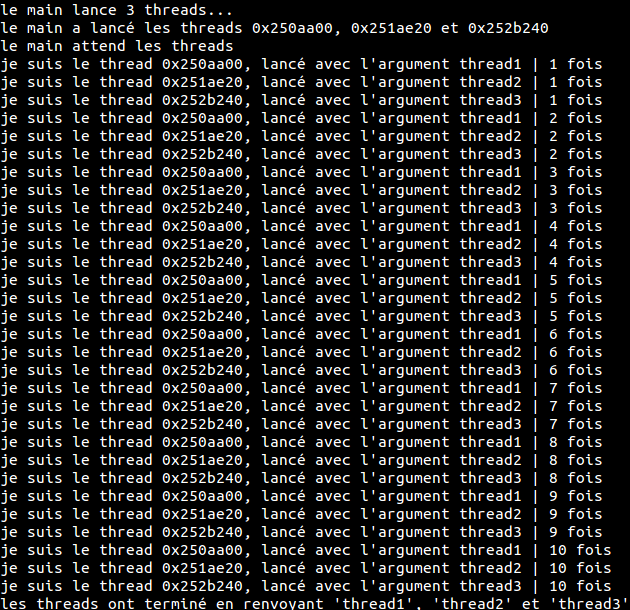
\includegraphics[width=8cm]{fifo.png}
      \caption{Ordonnancement FIFO}
      \label{fifo}
    \end{center}
  \end{minipage}
  \hfill
  \begin{minipage}[c]{.45\linewidth}
    \begin{center}
      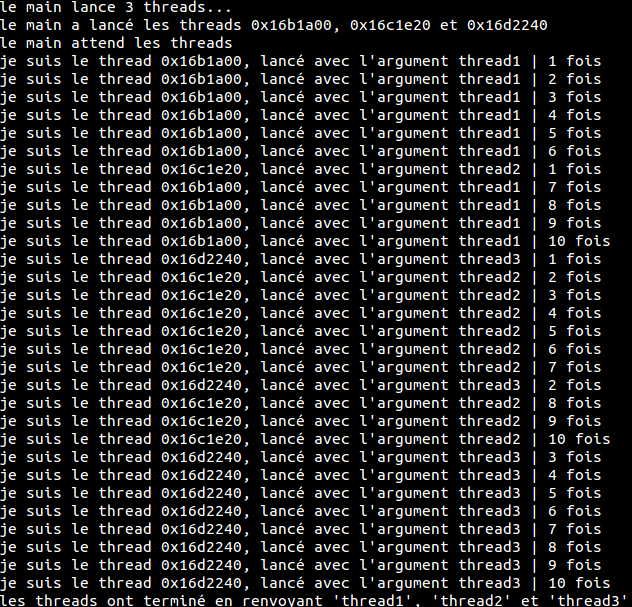
\includegraphics[width=8cm]{prio.png}
      \caption{Ordonnancement priorité}
      \label{prio}
    \end{center}
  \end{minipage}
\end{figure}


\section{Préemption}
Nous avons mis en place un préemption pseudo-coopérative, cachée dans
certaines fonctions de notre bibliothèque, de telle sorte que, au bout
d'une certaine durée prédéfinie, le thread en cours d'exécution reçoit
un signal \verb$SIGVTALRM$ et laisse la main au thread suivant dans la
liste "ready".

Cette forme de préemption est basée sur l'utilisation d'un timer, par
l'intermédiaire des fonctions \verb$setitimer$ et
\verb$getitimer$. Nous utilisons un timer virtuel, qui décroit
uniquement lorsque le processus s'exécute, et émet un signal
\verb$SIGVTALRM$ à l'expiration du délai.  La durée du timer est
définie par la variable globale \verb$TIMESLICE$.

Le timer est créé lors de la création du premier thread du programme,
et est désactivé lors de la disparition de ce même thread. Il est
réinitialisé dans \verb$thread_yield$, \verb$thread_join$ et
\verb$thread_exit$, pour que le thread qui reprend la main ait à son
tour le temps d'exécution disponible correspondant à la valeur de
\verb$TIMESLICE$. 

Dans notre version, nous avons donné à la variable \verb$TIMESLICE$
une valeur fixée, mais nous pourrions aller plus loin en lui donner
une valeur variable en fonction de la priorité du thread qui doit
s'exécuter.

\section{Communication à l'aide de signaux}
	Afin de permettre aux threads d'interagir entre eux, nous
        avons ajouté un système de signaux.  Ces signaux se
        représentent sous la forme d'entiers positifs qui sont stockés
        dans une liste dans la structure du thread. Ils peuvent être
        envoyés grâce à la fonction $thread\_kill$ prenant un
        paramètre un $thread\_t$ représentant le thread auquel envoyer
        le signal et un $int$ représentant le signal à envoyer.\\
	
	Ces signaux sont traités lors du passage au sein d'une des
        fonctions de la librairie, lors de son retour en exécution,
        l'ordonnanceur va effectuer les traitements de tous les
        signaux dans l'ordre de leur réception pendant que le thread
        était dans la file d'attente. Il y a pour le moment 6 signaux
        définis, un pour faire s'interrompre le thread, un autre, pour
        lui faire passer la main et les 4 autres sont des signaux
        personnalisables.\\
	
	Nous avons de plus permis de personnaliser le traitement de
        certains signaux, à l'aide d'une table de signaux propre à
        chaque thread. Cette table est renseignée à l'aide de la
        fonction $thread\_signal$ prenant en paramètre le thread à
        modifier, le signal auquel attribuer la fonction et un
        pointeur de fonction de signature $void(*func)(int)$ qui sera
        la fonction appelée lorsque le thread recevra le signal.\\
	
	Le programme $test\_signal$ teste l'implémentation de ces
        signaux. Il crée un thread qui fait deux boucles while, la
        première laissant la main à chaque tour et s'arrêtant
        lorsqu'il reçoit le signal $SIG\_USR1$, la seconde ne faisant
        rien. Ce thread reçoit à la suite un signal $SIG\_USR1$ et
        $SIG\_KILL$, on remarque dans l'exécution que le signal
        $SIG\_KILL$ est traité avant la sortie de la première
        boucle.\\


	Nous avons par la suite implémenté la possibilité aux threads
        d'envoyer des signaux à l'ordonnanceur concernant certains
        threads à l'aide de la fonction $thread\_signal$ sauf que les
        signaux envoyés sont alors des entiers négatifs. Ainsi nous
        avons défini deux signaux ordonnanceurs, un pour demander la
        suspension de l'exécution d'un thread actuellement dans un
        état exécutable, et un autre pour le remettre dans la liste
        des threads exécutables.\\
	
	Cette fonctionnalité est testée par le programme
        $test\_sig\_ordo$ qui exécute deux threads parallèles
        affichant les nombres de 1 à 10 tout en laissant la main entre
        chaque, mais l'un des threads va envoyer un signal à
        l'ordonnanceur pour retirer l'autre va finir de compter et va
        demander à l'ordonnanceur de remettre le thread dans la liste
        des threads exécutables.\\

\input{conclusion.tex}


%% \section{La mémoire}
%% Pour l'instant aucune libération de mémoire n'est faite. En
%% particulier nous ne nous sommes pas encore posé la question de quand
%% libérer les threads de la liste zombie. Cela pose un problème
%% évident lorsque le nombre de threads devient important. Nous nous
%% attellerons donc en priorité à la résolution de ce problème.

%% \section{Améliorations prévue}
%% Nous avons implémenté les programmes parallèles du calcul de la suite
%% de Fibonacci et de la somme des élément d'un tableau par
%% diviser-pour-régner. Cela nous permettra de tester les performances de
%% notre bibliothèque, en évaluant le temps d'exécution en fonction de la
%% taille de l'entrée. Il nous semble que la gestion du thread principal
%% est déjà prise en compte, il conviendra de s'en assurer. Nous pensons
%% mettre au point des fonctions de synchronisation de type
%% sémaphore. Nous aimerions aussi nous pencher sur la gestion de la
%% préemption et des signaux.

\end{document}
